\documentclass[a4,12pt]{book}
\usepackage{amsmath,amssymb}

\usepackage{geometry}
\geometry{
textwidth=157mm,
paperwidth=196mm,
paperheight=280mm,
top=1in,
left=27mm,
footskip=.7in
}

% Para enumerates customizados
\usepackage{enumerate}

% Para usar tabelas balanceadas
\usepackage{tabulary}

% Place crop marks
\usepackage[center,height=297mm,width=210mm,cam]{crop}

% Choose font
\usepackage{ifxetex}
\ifxetex
   \usepackage{fontspec}
   \setmainfont{Lato Light}
   \newfontface\titlefont{STIXIntegralsUp}
   \newfontface\thickfont{Nimbus Sans L}
   \newfontface\bigtitlefont[Scale=1.3]{Cabin}
   %\newcommand\titlefont{}
   %\newcommand\thickfont{}
\else
   \usepackage[utf8]{inputenc}
%   \usepackage[sfdefault,thin]{roboto}  %% sfdefault is the base font
   \newcommand\titlefont{\fontfamily{helvet}\selectfont}
   \newcommand\thickfont{\fontfamily{cmss}\selectfont}
   \newcommand\bigtitlefont{\fontfamily{cmss}\selectfont}
\fi

% Larger spacing between lines
\linespread{1.2}

% Temporary library for generating random text
\usepackage{lipsum}

% To define colors
\usepackage[dvipsnames]{xcolor}
\definecolor{titleblue}{RGB}{21,101,175}
\definecolor{myblue}{RGB}{204,216,241}
\definecolor{mediumblue}{RGB}{108,153,215}
\definecolor{myred}{RGB}{210,32,39}
\definecolor{mygreen}{RGB}{179,220,47}


% use o GIMP para obter o cógigo HTML da cor e o site a seguir para converter para RGB
% http://www.yellowpipe.com/yis/tools/hex-to-rgb/color-converter.php


% \usepackage{lastpage} % Required to determine the last page for the footer

% Pacotes para desenhos
\usepackage{tikz}
\usetikzlibrary{shapes}
\usetikzlibrary{calc}
% This package provides special PGF/TikZ nodes for the text, marginpar, footer and header area of the current page.
\usepackage{tikzpagenodes}
\tikzset{x=1mm,y=1mm}

%%%%%%%%%%%%%%%%%%%% Chapter and section titles %%%%%%%%%%%%%%%%%%%%%%%%%
\usepackage[explicit]{titlesec} % needed for define chapter and section style.
\setcounter{chapter}{1}
%%%%%%%%%%%%%%%%%%%%%%%%%%%%%%%%%%%%%%%%%%%%%%%%%%%%%%
\usepackage{titling}

% Chapter
\titleformat{\chapter} % redefining chapter appearence
%{} % style
{\titlefont\Huge\bf} % style
{} % label
{0pt} % separation
{\begin{tikzpicture}[remember picture,overlay]
    \filldraw [x=1mm,y=1mm, mygreen, overlay] (37,0) circle [radius=9];
    \filldraw [x=1mm,y=1mm, myred, overlay] (58,0) circle [radius=9];
    \filldraw [x=1mm,y=1mm, titleblue, overlay] (79,0) circle [radius=9];
    \filldraw [x=1mm,y=1mm, mediumblue, overlay] (210,-9) -- (100 ,-9) arc (-90:-270:9) --(100,9)
    -- (210,9) (118, 0) node{\color{white} Lição \thechapter} (105,-27);
  \end{tikzpicture}
} % before title
[\vspace{3cm} \hfill {\bf\bigtitlefont \color{mygreen} #1}] % after title
%\titlespacing*{\chapter}{0pt}{50pt}{100pt} % {<command>}{<left>}{<before-sep>}{<after-sep>}

% Section style %%%%%%%%%%%%%%%%%%%%%%%%%%%%%%%%
%\newcommand*\sectionlabel{}
\titleformat{\section}
  {\titlefont\bf}
  {\gdef\sectionlabel{\thesection\ }}{0pt}
  {%
    \begin{tikzpicture}[remember picture,overlay]
      \filldraw [x=1mm,y=1mm, myred, overlay] (\textwidth,-4) -- (0 ,-4)
      arc (-90:-270:4) --(0,4) -- (\textwidth,4)
      node[anchor=west] at (0, 0) {\color{white} \MakeUppercase{#1}};
   \end{tikzpicture}
 }
\titlespacing*{\section}{0pt}{20pt}{20pt} % {<command>}{<left>}{<before-sep>}{<after-sep>}
%%%%%%%%%%%%%%%%%%%%%%%%%%%%%%%%%%%%%%%%%%%%%%%%%%%%%%%%%%%%%%%%%%%%%%%%%%

% Subection style %%%%%%%%%%%%%%%%%%%%%%%%%%%%%%%%
\titleformat{\subsection}{\titlefont\Huge\bf\blue #1} % style
{} % label
{0pt} % separation

%%%%%%%%%%%%%%%%%%%%%%%%%%%%%%%%%%%%%%%%%%%%%%%%%%%%%%%%%%%%%%%%%%%%%%%%%%



%%%%%%%%%%%%%%%%%%%%%%% Custom headers and footers %%%%%%%%%%%%%%%%%%%%%%%
\usepackage{extramarks} % Required for headers and footers
\usepackage{fancyhdr}
\pagestyle{fancy}

% Chapter mark
\renewcommand{\chaptermark}[1]{\markboth{\ #1}{}}
% documentation abaout chaptermark, markboth, etc. https://www.ntg.nl/maps/16/29.pdf

% Section mark
\renewcommand{\sectionmark}[1]{\markright{\ #1}{}} % Sections not in uppercase, not numbered

% Footers
\fancyfoot[C]{%
\noindent%
\tikz[baseline]{\draw[color=ref, line width=0.6pt] (-0.5, 0) -- (6, 0);}%
}

% Left footer
\fancyfoot[LE]{
  {\tikz{\draw[color=myred, line width=0.6pt] (-1.8, 0) -- (\textwidth, 0);}}\newline
  {\tikz[x=1mm,y=1mm]{\filldraw [myred, overlay] (-20,-3) -- (-5 ,-3)
      arc (-90:90:3) --(-5,3) -- (-20,3) (-8, 0) node{\color{white} {\bf \thepage}};}}
  {\small\color{gray} Capítulo \thechapter \, - \, \leftmark}
}

% Right footer
\fancyfoot[RO]{
  {\tikz{\draw[color=myred, line width=0.6pt] (-1.8, 0) -- (\textwidth, 0);}}\newline
  {\small\color{gray} \rightmark}
  {\tikz[x=1mm,y=1mm]{\filldraw [myred, overlay] (20,-3) -- (5 ,-3)
      arc (-90:-270:3) --(5,3) -- (20,3) (8, 0) node{\color{white} {\bf \thepage}};}}
}%
\fancyfoot[C]{}

% Header
% Clear all header fields
\fancyhead{}
% No header rule
\renewcommand{\headrulewidth}{0pt}
%%%%%%%%%%%%%%%%%%%%%%%%%%%%%%%%%%%%%%%%%%%%%%%%%%%%%%%%%%%%%%%%%%%%%%%%%%%

%%%%%%%%%%%%%%%%%%%%%% Cabeçalho %%%%%%%%%%%%%%%%%%%%%%%%%%%%%%%%%%%%%%%%%%
\newcommand\Header{%
\begin{tikzpicture}[remember picture,overlay]
%\fill[myblue]
%  ([yshift=1mm]current page.north west) -- (current page.north east) --
%  ([yshift=0.3cm]current page.north east|-current page text area.north east) --
%  ([yshift=0.3cm]current page.north west|-current page text area.north west) -- cycle;
\fill[fill=myblue]
  ([yshift=2mm,xshift=-2mm]current page.north west) rectangle ([yshift=-5mm,xshift=2mm]current page.north east);
%\node[font=\sffamily\bfseries\color{white},anchor=east, % Texto dentro do cabeçalho acima
  xshift=-1.5cm,yshift=-1.3cm] at (current page.north east)
 % {\fontsize{50}{60}\selectfont  };
\end{tikzpicture}%
}
% This package provides various commands to be executed before a \shipout
\usepackage{atbegshi}
\AtBeginShipout{\Header}
\AtBeginShipoutFirst{\Header}
%%%%%%%%%%%%%%%%%%%%%%%%%%%%%%%%%%%%%%%%%%%%%%%%%%%%%%%%%%%%%%%%%%%%%%%%%%%


%%%%%%%%%%%%%%%%%%%%%% Ambientes %%%%%%%%%%%%%%%%%%%%%%%%%%%%%%%%%%%%%%%%%%
% Permite quebrar o tikz dentro da definição de um novo ambiente- como refletindo:
% http://tex.stackexchange.com/questions/5639 para explicação detalhada.
\usepackage{environ}

% % Atividade
% \newcounter{atividade}
% \newenvironment{atividade}[1][]{\refstepcounter{atividade}\par\medskip
%    \noindent \textbf{\textcolor{titleblue}{Atividade~\theatividade #1 \rmfamily \rmfamily}}}{\medskip}
%%%%%%%%%%%%%%%%%%%%%%%%%%%%%%%%%%%%%%%%%%%%%%%%%%

% Refletindo
\usepackage{tcolorbox}
%\usepackage{varwidth}
\tcbuselibrary{listings,breakable,most}
\newtcolorbox{refletindo*}[2][]{%
colframe=myblue,
colbacktitle=white,
coltitle=titleblue,
boxed title style={arc=3mm,boxrule=.7mm,height=8mm,valign=center},
enhanced,colback=white,
boxrule=.7mm,titlerule=3mm,
attach boxed title to top left={yshift=-2mm,xshift=3mm},
arc=4mm,
breakable,
fontupper=\thickfont,
title={\bf REFLETINDO},#1}
%%%%%%%%%%%%%%%%%%%%%%%%%%%%%%%%%%%%%%%%%%%%%%%%%%

\newtcbtheorem{professor}{Para o Professor}%
{colback=purple!15,colframe=purple,fonttitle=\bfseries}{th}
\newtcbtheorem{introdutorio}{Introdutório}%
{colback=green!5,colframe=green!35!black,fonttitle=\bfseries}{th}
\newtcbtheorem{abstrato}{Modelo abstrato}%
{colback=green!5,colframe=green!35!black,fonttitle=\bfseries}{th}
\newtcbtheorem{conexoes}{Conexões}%
{colback=green!5,colframe=green!35!black,fonttitle=\bfseries}{th}
\newtcbtheorem{explorando}{Explorando}%
{colback=green!5,colframe=green!35!black,fonttitle=\bfseries}{th}
\newtcbtheorem{massa}{Mão na massa}%
{colback=green!5,colframe=green!35!black,fonttitle=\bfseries}{th}
\newtcbtheorem{exercicio}{Exercício}%
{colback=gray!15,colframe=gray,fonttitle=\bfseries}{th}
\newtcbtheorem{resposta}{Resposta}%
{colback=blue!5,colframe=blue,fonttitle=\bfseries}{th}
\newtcbtheorem{imagem}{Imagem}%
{colback=yellow!15,colframe=yellow,fonttitle=\bfseries}{th}
\newtcbtheorem{figura}{Figura}%
{colback=green!5,colframe=green!35!black,fonttitle=\bfseries}{th}
\newtcbtheorem{nota}{Nota}%
{colback=gray!5,colframe=gray!35!black,fonttitle=\bfseries}{th}

\begin{document}

\chapter{ LIÇÃO 1 - Começando a falar sobre frações }


\includegraphics[width=\textwidth,height=4cm, keepaspectratio]{/var/www/livro/data/gitrepo/media/anchor/prologo}










\section{ EXPLORANDO O ASSUNTO }


\includegraphics[width=\textwidth,height=4cm, keepaspectratio]{/var/www/livro/data/gitrepo/media/anchor/ativ_equiparticao}

\subsection{ Atividade }







Três irmãos vão repartir uma barra de chocolate. Um deles sugere a seguinte divisão: 

\begin{imagem*}[breakable]{}{}   - FIGURA ARTÍSTICA   
  
  Na imagem devem estar 3 irmãos, aparentando idades diferentes (um deles pode ser cadeirante, por exemplo), observando uma única barra de chocolate retangular (preferencialemnte, imagem tridimensional sem subdivisões) repartida em três partes com tamanhos diferentes. Por exemplo:  
  
    \includegraphics[width=180pt, keepaspectratio]{/var/www/livro/data/gitrepo/media/cap1/secoes/licao1_1.png}  
  
\end{imagem*}

\begin{enumerate} [\quad a)] %d
  \item     Você concorda com essa divisão? Explique.
  \item     Com essa divisão, os três irmãos receberão a mesma quantidade de chocolate?
  \item     Use a imagem a seguir para mostrar uma divisão da barra de chocolate que permita que os 3 irmãos recebam quantidades iguais de chocolate. 
\end{enumerate} %d
\begin{imagem*}[breakable]{}{}    - FIGURA ARTÍSTICA - Inserir imagem da mesma barra retangular de chocolate da ilustração anterior sem qualquer partição sugerida. Apenas a imagem da barra de chocolate. Não há necessidade de ilustrar os irmãos.\end{imagem*}
\begin{enumerate} [\quad a)] %d
  \item     Considerando a divisão da barra de chocolate em 3 partes iguais, como você nomearia a quantidade de chocolate que cada irmão receberia? 
\end{enumerate} %d









\includegraphics[width=\textwidth,height=4cm, keepaspectratio]{/var/www/livro/data/gitrepo/media/anchor/ativ_equiparticao2}
\section{Atividade}







Três pizzas inteiras, de mesmo tamanho, foram repartidas entre as crianças de uma turma. Para isso, a turma foi dividida em três grupos com quatro crianças cada. Veja como cada grupo repartiu a sua pizza.

\begin{imagem*}[breakable]{}{}    - FIGURA ARTÍSTICA - A imagem deve conter 3 GRUPOS com 4 CRIANÇAS cada (Diversificar as características físicas das crianças). Cada um dos grupos deve estar observando uma pizza. Colocar duas das crianças do grupo 3 com feições   ``contrariadas''  . As pizzas devem ter mesmos tamanho e formato. As pizzas devem estar repartidas de três maneiras diferentes, como indicado nas imagens a seguir: Grupo 1, Grupo 2 e Grupo 3:   
  
    \includegraphics[width=300pt, keepaspectratio]{/var/www/livro/data/gitrepo/media/cap1/secoes/licao1_atv2.png}  
  
  ilustração: Cambrainha  
  
\end{imagem*}

\begin{enumerate} [\quad a)] %d
  \item     Cada um dos três grupos repartiu a sua pizza na mesma quantidade de fatias que os outros grupos?
  \item     Dessa maneira, todas as crianças da turma receberam a mesma quantidade de pizza?
  \item     Em algum dos grupos as 4 crianças receberam a mesma quantidade de pizza? Se sim, em qual? Considerando a pizza inteira, como você nomearia cada uma das fatias de pizza desse grupo? 
\end{enumerate} %d







\includegraphics[width=\textwidth,height=4cm, keepaspectratio]{/var/www/livro/data/gitrepo/media/anchor/ativ_enfeite}
\section{Atividade}







Alice quer enfeitar a sala de aula e pretende prender os enfeites utilizando pedaços de barbante. Para isso, quer cortar o barbante em pedaços iguais, para que os enfeites fiquem todos da mesma altura. Ajude Alice a cortar o barbante.

\begin{imagem*}[breakable]{}{}    - FIGURA ARTÍSTICA - Incluir imagem de um pedaço de barbante e de 4 estrelas congruentes, como ilustrado a seguir:  
  Alice é uma menina morena de rabo de cavalo. Ela será um personagem frequente deste livro.  
  
    \includegraphics[width=180pt, keepaspectratio]{/var/www/livro/data/gitrepo/media//cap1/secoes/alice_barbante_estrelas.jpg}  
\end{imagem*}

\begin{imagem*}[breakable]{}{}   - FIGURA ARTÍSTICA -  
  \begin{nota*}[breakable]{}{}         
    INCLUIR PÁGINA DE REPRODUÇÃO COM apenas 1 ESTRELA com aproximadamente 10 cm de altura para ser recortada.    
  \end{nota*}  
\end{imagem*}






\includegraphics[width=\textwidth,height=4cm, keepaspectratio]{/var/www/livro/data/gitrepo/media/anchor/conexoes}

\chapter{ ORGANIZANDO AS IDEIAS }


  


Os números que você havia estudado até aqui são usados para contar, ordenar e rotular, e são chamados números naturais.
\begin{imagem*}[breakable]{}{}   - FIGURA ARTÍSTICA - ESTA IMAGEM PRECISA SER REFEITA.  
    \includegraphics[width=360pt, keepaspectratio]{/var/www/livro/data/gitrepo/media//cap1/secoes/numeros-naturais-01.png}  
\end{imagem*}

Para que servem os números naturais?

As atividades que foram apresentadas nesta lição lidam com quantidades não inteiras: um terço de uma barra de chocolate, um quarto de pizza, por exemplo. 
Outros exemplos aparecem no nosso dia a dia: ``o ser humano passa um terço de sua vida dormindo'', ``eu tomei a metade de um copo de leite''. 
Nas atividades que realizamos, uma barra de chocolate, pizzas e um pedaço de barbante foram repartidos em partes iguais. 
Nesses casos, a barra de chocolate, uma pizza e o pedaço de barbante são vistos como unidades. 
Cada uma das partes em que essas unidades foram repartidas igualmente é uma fração da unidade.

\begin{imagem*}[breakable]{}{}   - FIGURA ARTÍSTICA -  
  {\bf Imagem de uma pizza e de um pedaço de barbante, cada um dividido em 4 partes.}  
\end{imagem*}

O nome dado à fração da unidade depende da quantidade de partes em que a unidade é dividida. 

Ao dividir uma unidade qualquer em duas partes iguais ou ao meio, cada uma das partes é chamada de {\it um meio} ou {\it a metade} da unidade. 

Por exemplo, se uma barra de chocolate é repartida igualmente entre dois amigos, a quantidade que caberá a cada um dos amigos é {\it um meio} da barra de chocolate (ou {\it metade} da barra). Nesse exemplo, a unidade é a barra de chocolate.

\begin{imagem*}[breakable]{}{}   - FIGURA ARTÍSTICA - INCLUIR IMAGENS ILUSTRATIVA de metade   
  {\bf Imagem de duas crianças a barra de chocolate em que a metade é identificada}  
\end{imagem*}

Ao dividir uma unidade em três partes iguais, cada uma das partes é chamada de {\it um terço} ou {\it a terça parte} da unidade. 

Por exemplo, se, em uma receita de bolo, é necessário acrescentar {\it um terço} de um litro de leite. Isso significa que, para colocar a quantidade correta de leite na receita, é preciso repartir o litro de leite em três partes iguais e usar apenas uma dessas partes, que é {\it um terço} do litro de leite. Nesse caso, a unidade é um litro de leite.

\begin{imagem*}[breakable]{}{}   - FIGURA ARTÍSTICA - INCLUIR IMAGEM ILUSTRATIVA de terço   
  {\bf Sobre uma mesa, uma garrafa cilindrica cheia de leite e três garrafas iguais ao lado, cada uma com 1/3 da capacidade prennchida.}  
  
  Por exemplo:   
    \includegraphics[width=60pt, keepaspectratio]{/var/www/livro/data/gitrepo/media//cap1/secoes/litro_de_leite.jpg}  
    \includegraphics[width=60pt, keepaspectratio]{/var/www/livro/data/gitrepo/media//cap1/secoes/um_terco_de_litro_de_leite.jpg}  
  
\end{imagem*}

Ao dividir uma unidade em quatro partes iguais, cada uma das partes é chamada de {\it um quarto} ou {\it quarta parte} da unidade. 

Por exemplo,
A parte colorida da figura é um quarto da figura. Neste caso, a figura é a unidade.


\begin{imagem*}[breakable]{}{}   - FIGURA ARTÍSTICA - INCLUIR IMAGEM ILUSTRATIVA de quartos  
    \includegraphics[width=120pt, keepaspectratio]{/var/www/livro/data/gitrepo/media//cap1/secoes/quartos_conexoes.jpg}  
   \end{imagem*}

Da mesma forma, ao dividir uma unidade em cinco partes iguais, cada uma das partes é chamada de {\it um quinto} ou {\it quinta parte} da unidade.

Por exemplo,
{\it um quinto} de todo ouro pesado nas Casas de Fundição no Brasil era pago em impostos à Coroa Portuguesa. Desta forma, a quantidade de ouro pago em impostos à Coroa Portuguesa era igual a {\it um quinto} ou a {\it quinta parte} do ouro pesado nas Casas de Fundição no Brasil.

\begin{imagem*}[breakable]{}{}   - FIGURA ARTÍSTICA - INCLUIR IMAGEM ILUSTRATIVA de quintos   
  {\bf Um homem entregando um saco de ouro a um rei e ficando com outros 4 sacos}  
\end{imagem*}









\chapter{ MÃO NA MASSA }


\includegraphics[width=\textwidth,height=4cm, keepaspectratio]{/var/www/livro/data/gitrepo/media/anchor/ativ_retangulos_coloridos}
\section{Atividade}







Quais dos retângulos a seguir foram repartidos em {\it quartos}?

\begin{imagem*}[breakable]{}{}   - FIGURA GEOMÉTRICA - A imagem deve conter oito retângulos   {\bf congruentes}   coloridos, cada um com uma cor diferente das demais. Os retângulos devem estar divididos em partes conforme a imagem   
    \includegraphics[width=120pt, keepaspectratio]{/var/www/livro/data/gitrepo/media//cap1/secoes/quartos.jpg}  
  
\end{imagem*}










\includegraphics[width=\textwidth,height=4cm, keepaspectratio]{/var/www/livro/data/gitrepo/media/anchor/refl_retangulos_coloridos}



\begin{refletindo*}[breakable]{}{}  
  Quando se diz que uma unidade é repartida em meios, terços, quartos, quintos, etc., a unidade foi repartida em 2, 3, 4, 5, etc. partes de mesma quantidade.  
  Na atividade acima, se os retângulos representam bolos (ou barras de chocolate), as quatro partes em que foram divididos os retângulos possuem mesma quantidade de bolo (ou de chocolate).  
  Os retângulos foram divididos em quartos, embora as partes não possuam mesma forma.  
\end{refletindo*}


\includegraphics[width=\textwidth,height=4cm, keepaspectratio]{/var/www/livro/data/gitrepo/media/anchor/ativ_ident_terco}
\section{Atividade}








Em cinco das figuras a seguir a parte em vermelho é um terço da figura. Identifique estas figuras.
\begin{imagem*}[breakable]{}{}   - FIGURA GEOMÉTRICA - Estas figuras devem ser produzidas individualmente, importante levar em conta a fração. Não se deve colocar os itens A), B), etc.  
    \includegraphics[width=300pt, keepaspectratio]{/var/www/livro/data/gitrepo/media//cap1/secoes/um_terco_vermelho.jpg}  
\end{imagem*}







\includegraphics[width=\textwidth,height=4cm, keepaspectratio]{/var/www/livro/data/gitrepo/media/anchor/ativ_recomportodo}
\section{Atividade}







\begin{imagem*}[breakable]{}{}   FIGURAS GEOMÉTRICAS - As figuras das linhas devem ser feitas individualmente. Observe que há figuras no   ``Para o professor''   e na   ``Resposta''  .  
\end{imagem*}
\begin{enumerate} [\quad a)] %s
  \item     
\end{enumerate} %s
\includegraphics[width=18pt, keepaspectratio]{/var/www/livro/data/gitrepo/media/undefined/completar-o-todo-disco.jpg} é metade de uma figura. Complete a figura para obter a unidade.
\begin{enumerate} [\quad a)] %s
  \item     
\end{enumerate} %s
\includegraphics[width=18pt, keepaspectratio]{/var/www/livro/data/gitrepo/media/undefined/completar-o-todo-disco.jpg} é um terço de uma figura. Complete a figura para obter a unidade.
\begin{enumerate} [\quad a)] %s
  \item     
\end{enumerate} %s
\includegraphics[width=18pt, keepaspectratio]{/var/www/livro/data/gitrepo/media/undefined/completar-o-todo-disco.jpg} é um quarto de uma figura. Complete a figura para obter a unidade.
\begin{enumerate} [\quad a)] %s
  \item     
\end{enumerate} %s
\includegraphics[width=18pt, keepaspectratio]{/var/www/livro/data/gitrepo/media/undefined/completar-o-todo-quadrado.jpg} é metade de uma figura. Complete a figura para obter a unidade.
\begin{enumerate} [\quad a)] %s
  \item     
\end{enumerate} %s
\includegraphics[width=18pt, keepaspectratio]{/var/www/livro/data/gitrepo/media/undefined/completar-o-todo-quadrado.jpg} é um terço de uma figura. Complete a figura para obter a unidade.
\begin{enumerate} [\quad a)] %s
  \item     
\end{enumerate} %s
\includegraphics[width=18pt, keepaspectratio]{/var/www/livro/data/gitrepo/media/undefined/completar-o-todo-quadrado.jpg} é um quarto de uma figura. Complete a figura para obter a unidade.
\begin{enumerate} [\quad a)] %s
  \item     
\end{enumerate} %s
\includegraphics[width=18pt, keepaspectratio]{/var/www/livro/data/gitrepo/media/undefined/completar-o-todo-segmento.jpg} é metade de uma figura. Complete a figura para obter a unidade.
\begin{enumerate} [\quad a)] %s
  \item     
\end{enumerate} %s
\includegraphics[width=18pt, keepaspectratio]{/var/www/livro/data/gitrepo/media/undefined/completar-o-todo-segmento.jpg} é um terço de uma figura. Complete a figura para obter a unidade.
\begin{enumerate} [\quad a)] %s
  \item     
\end{enumerate} %s
\includegraphics[width=18pt, keepaspectratio]{/var/www/livro/data/gitrepo/media/undefined/completar-o-todo-segmento.jpg} é um quarto de uma figura. Complete a figura para obter a unidade.
\begin{enumerate} [\quad a)] %s
  \item     
\end{enumerate} %s
\includegraphics[width=24pt, keepaspectratio]{/var/www/livro/data/gitrepo/media/undefined/completar-o-todo-triangulo.jpg} é metade de uma figura. Complete a figura para obter a unidade.
\begin{enumerate} [\quad a)] %s
  \item     
\end{enumerate} %s
\includegraphics[width=24pt, keepaspectratio]{/var/www/livro/data/gitrepo/media/undefined/completar-o-todo-triangulo.jpg} é um terço de uma figura. Complete a figura para obter a unidade.
\begin{enumerate} [\quad a)] %s
  \item     
\end{enumerate} %s
\includegraphics[width=24pt, keepaspectratio]{/var/www/livro/data/gitrepo/media/undefined/completar-o-todo-triangulo.jpg} é um quarto de uma figura. Complete a figura para obter a unidade.





\includegraphics[width=\textwidth,height=4cm, keepaspectratio]{/var/www/livro/data/gitrepo/media/anchor/ativ_desenhar}
\section{Atividade}






\begin{imagem*}[breakable]{}{}   FIGURAS GEOMÉTRICAS - Observe que há figuras no   ``Para o professor''   e na   ``Resposta''  .  
\end{imagem*}

\begin{enumerate} [\quad a)] %d
  \item     Pinte metade do quadrado a seguir.
\end{enumerate} %d
\mbox{} \newline  \includegraphics[width=150pt, keepaspectratio]{/var/www/livro/data/gitrepo/media//cap1/secoes/um-meio-um-quarto-um-oitavo.jpg}
\begin{enumerate} [\quad a)] %d
  \item     Pinte um quarto do quadrado a seguir.
\end{enumerate} %d
\mbox{} \newline  \includegraphics[width=150pt, keepaspectratio]{/var/www/livro/data/gitrepo/media//cap1/secoes/um-meio-um-quarto-um-oitavo.jpg}
\begin{enumerate} [\quad a)] %d
  \item     Pinte um oitavo do quadrado a seguir.
\end{enumerate} %d
\mbox{} \newline  \includegraphics[width=150pt, keepaspectratio]{/var/www/livro/data/gitrepo/media//cap1/secoes/um-meio-um-quarto-um-oitavo.jpg}
\begin{enumerate} [\quad a)] %d
  \item     Observando os quadrados acima pintados. Qual é a maior das frações do quadrado: metade, quarto ou oitavo?
\end{enumerate} %d






\includegraphics[width=\textwidth,height=4cm, keepaspectratio]{/var/www/livro/data/gitrepo/media/anchor/ativ_hexag}
\section{Atividade}






\begin{imagem*}[breakable]{}{}   FIGURAS GEOMÉTRICAS - As figuras das linhas devem ser feitas individualmente. Observe que também há figuras na   ``Resposta''  .  
\end{imagem*}
\begin{enumerate} [\quad a)] %d
  \item     Pinte metade da figura. 
\end{enumerate} %d
\mbox{} \newline  \includegraphics[width=90pt, keepaspectratio]{/var/www/livro/data/gitrepo/media//cap1/secoes/fracoes-unitarias-dois-hexagonos-03.jpg}
\begin{enumerate} [\quad a)] %d
  \item     Pinte metade da figura de forma diferente do item anterior. 
\end{enumerate} %d
\mbox{} \newline  \includegraphics[width=90pt, keepaspectratio]{/var/www/livro/data/gitrepo/media//cap1/secoes/fracoes-unitarias-dois-hexagonos-03.jpg}
\begin{enumerate} [\quad a)] %d
  \item     Pinte a metade da figura de forma diferente dos três anteriores. 
\end{enumerate} %d
\mbox{} \newline  \includegraphics[width=90pt, keepaspectratio]{/var/www/livro/data/gitrepo/media//cap1/secoes/fracoes-unitarias-dois-hexagonos-03.jpg}







\includegraphics[width=\textwidth,height=4cm, keepaspectratio]{/var/www/livro/data/gitrepo/media/anchor/ativ_meioemeio}
\section{Atividade}








Identique as figuras em que a parte pintada é a metade da figura.
\begin{imagem*}[breakable]{}{}    FIGURAS GEOMÉTRICAS - As figuras devem ser feitas individualmente. As dimensões para a página de reprodução são: retângulos 10 por 3 cm, círculo de raios 3 cm e hexágonos de diâmetro 6 cm. Aqui elas podem ser um pouco menores para ficarem bem na página.  
    \includegraphics[width=\textwidth,height=4cm, keepaspectratio]{/var/www/livro/data/gitrepo/media//cap1/secoes/1_10_meio_e_meio.jpg}  
\end{imagem*}










\includegraphics[width=\textwidth,height=4cm, keepaspectratio]{/var/www/livro/data/gitrepo/media/anchor/ativ_variadas}
\section{Atividade}







Considere o círculo como unidade. 
\begin{enumerate} [\quad a)] %s
  \item      Que afirmação corresponde à parte colorida em cada uma das figuras?  
\end{enumerate} %s
\mbox{} \newline 
\begin{enumerate} [\quad a)] %d
  \item    	A parte colorida é um quinto do círculo.
  \item    	A parte colorida é a sexta parte do círculo.
  \item    	A parte colorida é um sétimo do círculo.
  \item    	A parte colorida é um oitavo do círculo.
  \item    	A parte colorida é a nona parte do círculo.
  \item    	A parte colorida é um décimo do círculo.
\end{enumerate} %d
\mbox{} \newline  \begin{imagem*}[breakable]{}{}   FIGURAS GEOMÉTRICAS - As figuras devem ser feitas individualmente e não devem conter os itens A), B), etc.  
    \includegraphics[width=360pt, keepaspectratio]{/var/www/livro/data/gitrepo/media//cap1/secoes/circulos.jpg}  
\end{imagem*}\mbox{} \newline 
\begin{enumerate} [\quad a)] %s
  \item     Dentre as frações do círculo apresentadas, encontre uma que seja menor que um sexto do círculo.
  \item     Dentre as frações do círculo apresentadas, encontre uma que seja maior que um nono do círculo.
  \item     Encontre uma fração do círculo que seja menor que um sexto e maior que um nono do círculo.
\end{enumerate} %s







\includegraphics[width=\textwidth,height=4cm, keepaspectratio]{/var/www/livro/data/gitrepo/media/anchor/ativ_visual_linguagem}
\section{Atividade}










Em cada uma das imagens, a parte colorida é uma fração da figura. Essas frações podem ser ``um meio'', ``um quarto'' ou ``um décimo'' da figura. Associe cada imagem à fração correspondente.

\begin{imagem*}[breakable]{}{}   FIGURAS GEOMÉTRICAS - Devem ser feitas individualmente sem os itens A), B), etc.  
  
    \includegraphics[width=360pt, keepaspectratio]{/var/www/livro/data/gitrepo/media//undefined/ummeio_umquarto_um_decimo.jpg}  
  
  
\end{imagem*}










\end{document}